\documentclass{standalone}
\usepackage[english]{babel}
% https://tex.stackexchange.com/questions/570303/use-blacktriangleright-as-itemize-label
\usepackage{amssymb} % for black triangleright

\usepackage{amsmath}

\usepackage{graphicx}
% \graphicspath{figures/}

\renewcommand{\labelitemi}{$\textcolor{SwitchColor}{\bullet}$}
\renewcommand{\labelitemii}{$\textcolor{SwitchColor}{\blacktriangleright}$}
\renewcommand{\labelitemiii}{$\textcolor{SwitchColor}{\blacksquare}$}

% https://tex.stackexchange.com/questions/525959/prevent-latex-from-stretching-math
\setlength{\thinmuskip}{1\thinmuskip}
\setlength{\medmuskip}{1\medmuskip}
\setlength{\thickmuskip}{1\thickmuskip}

\usepackage{csquotes}
\usepackage{xcolor}
% \usepackage{anyfontsize}
\usepackage[export]{adjustbox}
% \usepackage[]{enumitem}
\usepackage{tikz}
\usetikzlibrary{arrows.meta,positioning}
\usetikzlibrary{graphs}
\usetikzlibrary{patterns}
\usetikzlibrary{shadings}
\usetikzlibrary{mindmap, shadows, backgrounds} % , calc

\definecolor{SecondaryColor}{HTML}{BBAF01}
\definecolor{SecondaryColorDimmed}{HTML}{FEF684}
\definecolor{PrimaryColor}{HTML}{E95112}
\definecolor{PrimaryColorDimmed}{HTML}{F6AF91}
\definecolor{SwitchColor}{named}{PrimaryColor}
\colorlet{BoxColor}{gray!10!white}

\usepackage[allbordercolors=PrimaryColor, pdfborder={0 0 .2}]{hyperref}

% colored bold
% \newcommand\alert[1]{\textcolor{SwitchColor}{\textbf{#1}}}
\newcommand\alert[1]{\textcolor{SwitchColor}{#1}}

\newlength{\leveldistance}
\setlength{\leveldistance}{25cm}

\begin{document}
  \begin{tikzpicture}[
      auto,
      huge mindmap,
      fill opacity=0.6,
      draw opacity=0.8,
      concept color = PrimaryColorDimmed,
      every annotation/.style={fill=BoxColor, draw=none, align=center, fill = BoxColor, text width = 2cm},
      grow cyclic,
      level 1/.append style = {
        concept color=SecondaryColorDimmed,
        level distance=\leveldistance,
        sibling angle=360/\the\tikznumberofchildren,
        % https://tex.stackexchange.com/questions/501240/trying-to-use-the-array-environment-inside-a-tikz-node-with-execute-at-begin-no
        execute at begin node=\definecolor{SwitchColor}{named}{SecondaryColor},
      },
      level 2/.append style = {
        concept color=PrimaryColorDimmed,
        level distance=\leveldistance / 2,
        sibling angle=30,
        execute at begin node=\definecolor{SwitchColor}{named}{PrimaryColor},
      },
      level 3/.append style = {
        concept color=SecondaryColorDimmed,
        level distance=\leveldistance / 3,
        execute at begin node=\definecolor{SwitchColor}{named}{SecondaryColor},
      },
      level 4/.append style = {
        concept color=PrimaryColorDimmed,
        level distance=\leveldistance / 4,
        execute at begin node=\definecolor{SwitchColor}{named}{PrimaryColor},
      },
      level 5/.append style = {
        concept color=SecondaryColorDimmed,
        level distance=\leveldistance / 5,
        execute at begin node=\definecolor{SwitchColor}{named}{SecondaryColor},
      },
      level 6/.append style = {
        concept color=PrimaryColorDimmed,
        level distance=\leveldistance / 6,
        execute at begin node=\definecolor{SwitchColor}{named}{PrimaryColor},
      },
      level 7/.append style = {
        concept color=SecondaryColorDimmed,
        level distance=\leveldistance / 7,
        execute at begin node=\definecolor{SwitchColor}{named}{SecondaryColor},
      },
      level 8/.append style = {
        concept color=PrimaryColorDimmed,
        level distance=\leveldistance / 8,
        execute at begin node=\definecolor{SwitchColor}{named}{PrimaryColor},
      },
      concept connection/.append style = {
        color = BoxColor,
      },
  ]
  % damit Annotationen nicht auch eine Drop Shadow erhalten
  \begin{scope}[
      every node/.style = {concept, circular drop shadow}, % draw=none
      every child/.style={concept},
    ]
  \node (gt) at (current page.center) {Graph Theory
      \resizebox{\textwidth}{!}{
        \begin{minipage}[t]{18cm}
          \begin{itemize}
            \item the order (germ. Knotenzahl) $n(G)$ of a graph $G$ is the number of vertices
            \item the size (germ. Kantenzahl) $e(G)$ of a graph $G$ is the number of edges
          \end{itemize}
        \end{minipage}
      }
    }
  child {
    node {Dual Problems}
            child {
              node {Chromatic number $\chi(G)$
                \resizebox{\textwidth}{!}{
                  \begin{minipage}[t]{8cm}
                    \begin{itemize}
                      \item is the \alert{minimum} number of colors such that \alert{adjacent vertices} receive \alert{different colors}
                    \end{itemize}
                  \end{minipage}
                }
              }
            }
    child {
      node {Min-Cut and Maximum-Flow
        \resizebox{\textwidth}{!}{
          \begin{minipage}[t]{8cm}
            \begin{itemize}
              \item coming later in the lecture
            \end{itemize}
          \end{minipage}
        }
      }
    }
    child {
      node {Matching and Vertex cover
        \resizebox{\textwidth}{!}{
          \begin{minipage}[t]{8cm}
            \begin{itemize}
              \item the  size of a \alert{vertex cover} is always at least as big as the size of a \alert{matching}
              \item \alert{Theorem (König und Egerváry):} For any bipartite graph $G$ the size of maximum matching equals the size of minimum vertex cover
            \end{itemize}
          \end{minipage}
        }
      }
      child {
        node {Matching
          \resizebox{\textwidth}{!}{
            \begin{minipage}[t]{8cm}
              \begin{itemize}
                \item a \alert{matching} $M$ in a graph $G$ is a set of non-loop edges with no shared endpoints
                \begin{itemize}
                  \item the vertices incident to the edges of a matching M are \alert{$M$-saturated}
                  \item the other vertices are \alert{$M$-unsaturated}
                  \item a \alert{perfect matching} saturates every vertex
                  \item the \alert{size} of a matching is given by the \alert{number of edges}
                  \item a \alert{maximal matching} in a graph is a matching that cannot be enlarged by adding an edge
                  \item a \alert{maximum matching} is a matching of maximum size (among all matchings in a graph)
                  \item $\alpha'(G)$ is the maximum size of matching of edges in $G$
                \end{itemize}
              \end{itemize}
            \end{minipage}
          }
        }
        child {
          node (mec) {Other Connections
            \resizebox{\textwidth}{!}{
              \begin{minipage}[t]{8cm}
                \begin{itemize}
                  \item \alert{Theorem(Gallai):} If G is a graph without isolated vertices, then $\alpha'(G) + \beta'(G) = n(G)$
                \end{itemize}
              \end{minipage}
            }
          }
        }
        child {
          node {Theorem (Berge)
            \resizebox{\textwidth}{!}{
              \begin{minipage}[t]{8cm}
                \begin{itemize}
                  \item a matching $M$ in a graph $G$ is a maximum matching in $G$ \alert{iff} $G$ has no $M$-augmenting path
                \end{itemize}
              \end{minipage}
            }
          }
          child {
            node (apa) {Augmenting Path Algorithm
              \resizebox{\textwidth}{!}{
                \begin{minipage}[t]{8cm}
                  \begin{itemize}
                    \item  Repeatedly applying the Augmenting Path Algorithm to a bipartite graph produces a \alert{matching} and a \alert{vertex cover} of equal size
                  \end{itemize}
                \end{minipage}
              }
            }
          }
          child {
            node {Alternating and Augmenting Paths
              \resizebox{\textwidth}{!}{
                \begin{minipage}[t]{8cm}
                  \begin{itemize}
                    \item given a matching $M$ in $G$, an \alert{$M$-alternating path} is a path that alternates between edges in $M$ and edges not in $M$
                    \item an $M$-alternating path whose endpoints are unsaturated by $M$ is an \alert{$M$-augmenting path}
                  \end{itemize}
                \end{minipage}
              }
            }
          }
        }
        child {
          node {Theorem (Hall)
            \resizebox{\textwidth}{!}{
              \begin{minipage}[t]{8cm}
                \begin{itemize}
                  \item An $X$, $Y$-bigraph has a matching that saturates $X$ if and only if $|N(S)| \ge |S|$ for all $S \subseteq X$
                \end{itemize}
              \end{minipage}
            }
          }
          child {
            node {X,Y-Bigraph
              \resizebox{\textwidth}{!}{
                \begin{minipage}[t]{8cm}
                  \begin{itemize}
                    \item a bipartite graph with vertex sets $X$ and $Y$ and edges only between $X$ and $Y$
                  \end{itemize}
                \end{minipage}
              }
            }
          }
        }
        child {
          node {Complete Graphs
            \resizebox{\textwidth}{!}{
              \begin{minipage}[t]{8cm}
                \begin{itemize}
                  \item $K_{2n}$ has $f_n = (2n-1)\cdot f_{n-1} = 1\cdot 3\cdot 5\cdot (2n-1)$ choices for choices for perfect matchings
                  \begin{itemize}
                    \item $K_n$ is a complete graph with $n$ vertices, i.e. a simple graph with maximum number of edges
                  \end{itemize}
                  \item $K_{2n+1}$ has no perfect matching because the node number of vertices is odd
                \end{itemize}
              \end{minipage}
            }
          }
        }
        child {
          node {Regular Bipartite graphs
            \resizebox{\textwidth}{!}{
              \begin{minipage}[t]{8cm}
                \begin{itemize}
                  \item for $k > 0$, every $k$-regular bipartite graph has a perfect matching
                \end{itemize}
              \end{minipage}
            }
          }
        }
        child {
          node {Symmetric Differences of Matchings
            \resizebox{\textwidth}{!}{
              \begin{minipage}[t]{8cm}
                \begin{itemize}
                  \item  Every component of the symmetric difference of two matchings
                  \begin{itemize}
                    \item is a path or
                    \item an even cycle
                  \end{itemize}
                \end{itemize}
              \end{minipage}
            }
          }
        }
      }
      child {
        node (vc) {Vertex cover
          \resizebox{\textwidth}{!}{
            \begin{minipage}[t]{8cm}
              \begin{itemize}
                \item a set $Q \subseteq V(G)$ that contains at least one endpoint of every edge
                \item the vertices $Q$ cover $E(G)$
                \begin{itemize}
                  \item $\beta(G)$ is the minimum size of vertex cover in $G$
                \end{itemize}
              \end{itemize}
            \end{minipage}
          }
        }
      }
    }
    child {
      node {Independence number and edge cover
        \resizebox{\textwidth}{!}{
          \begin{minipage}[t]{8cm}
            \begin{itemize}
              \item content
            \end{itemize}
          \end{minipage}
        }
      }
      child {
        node {Independence number
          \resizebox{\textwidth}{!}{
            \begin{minipage}[t]{8cm}
              \begin{itemize}
                \item Vertices are \alert{independent}, if they are not connected via an edge
                \begin{itemize}
                  \item $\alpha(G)$ is the maximum size of independent set of vertices in $G$
                \end{itemize} 
              \end{itemize}
            \end{minipage}
          }
        }
        child {
          node (isvc) {Other Connections
            \resizebox{\textwidth}{!}{
              \begin{minipage}[t]{8cm}
                \begin{itemize}
                  \item in a graph $G$ the set $S$ is an independent set \alert{iff} $\overline{S}$ is a vertex cover
                  \item $\alpha(G) + \beta(G) = n(G)$
                \end{itemize}
              \end{minipage}
            }
          }
        }
      }
      child {
        node (ec) {Edge cover 
          \resizebox{\textwidth}{!}{
            \begin{minipage}[t]{8cm}
              \begin{itemize}
                \item a set $L$ of edges such that every vertex of $G$ is incident to some edge of $L$
                \begin{itemize}
                  \item $\beta'(G)$ is the minimum size of edge cover in $G$
                \end{itemize}
              \end{itemize}
            \end{minipage}
          }
        }
      }
    }
  }
  child {
    node {(Undirected) Graphs $G = (V, E, R)$
      \resizebox{\textwidth}{!}{
        \begin{minipage}[t]{10cm}
          \begin{itemize}
            \item \alert{vertex set}, e.g. $V(G) = \{v_1, v_2, \ldots\}$
            \item \alert{edge set}, e.g. $E(G) = \{e_1, e_2, \ldots\}$
            \item \alert{relation}, e.g. $R(G) = \{(e_1, \{v_1, v_2\}), \ldots\}$ that associates with each \alert{edge} a set of two vertices, called its \alert{endpoints}
            \item a \alert{loop} is an edge with equal endpoints 
            \item \alert{multiple edges} are edges with same pair of endpoints                       
            \item \underline{\href[page=37]{/home/areo/Documents/Studium/Summaries/Graph_Theory/Graphentheorie_english_all_in_one_with_go_back.pdf}{interesting properties}:}
            \begin{itemize}
              \item $\displaystyle \sum_{v\in V(G)} d(v) = 2\cdot e(G)$
              \item in a graph $G$ the average vertex degree is $\displaystyle \frac{\sum_{v\in V(G)} d(v)}{\mathrm{n}(\mathrm{G})}$ and hence $\displaystyle \delta(G) \leq \frac{2 \cdot e(G)}{n(G)} \leq \Delta(G)$
              \item every graph has an even number of vertices of odd degree
              \item a $k$-regular graph with $n$ vertices has $\frac{n\cdot k}{2}$ edges
              \item the maximum number of edges in a simple graph is $\dbinom{n}{2}$
              \item the minimum number of edges in a connected graph with $n$ vertices is $n-1$
              \item if $G$ is a simple $n$-vertex graph with $\delta(G) \ge \dfrac{n-1}{2}$ then $G$ is connected
            \end{itemize}
          \end{itemize}
        \end{minipage}
      }
    }
    child {
      node {Trees
        \resizebox{\textwidth}{!}{
          \begin{minipage}[t]{12cm}
            \begin{itemize}
              \item a graph with no cycle is \alert{acyclic}
              \item a \alert{forest} is an acyclic graph
              \item a \alert{tree} is a connected acyclic graph
              \item a \alert{leaf} is a vertex of degree $1$
              \item \underline{\href[page=59]{/home/areo/Documents/Studium/Summaries/Graph_Theory/Graphentheorie_english_all_in_one_with_go_back.pdf}{interesting properties}}
                \begin{itemize}
                  \item every tree with at least two vertices has at least two leaves
                  \item deleting a leaf from an $n$-vertex tree produces a tree with $n-1$ vertices
                  \item for an $n$-vertex simple graph $G$ (with $n\ge 1$) the following are equivalent:
                    \begin{enumerate}
                      \item $G$ is connected and has no cycles
                      \item $G$ is connected and has $n-1$ edges
                      \item $G$ has $n-1$ edges and no cycles
                      \item for $u, v \in V(G)$, $G$ has exactly one $u, v$-path
                    \end{enumerate}
                  \item every edge of a tree is a cut-edge
                  \item adding one edge to a tree forms exactly one cycle
                \end{itemize}
            \end{itemize}
          \end{minipage}
        }
      }
      child {
        node {Spanning Trees
          \resizebox{\textwidth}{!}{
            \begin{minipage}[t]{12cm}
              \begin{itemize}
                \item a \alert{spanning subgraph} of $G$ is a subgraph with vertex set $V(G)$
                \item a \alert{spanning tree} is a spanning subgraph that is a tree
                \item \underline{\href[page=69]{/home/areo/Documents/Studium/Summaries/Graph_Theory/Graphentheorie_english_all_in_one_with_go_back.pdf}{interesting properties}:}
                  \begin{itemize}
                    \item every connected graph contains a spanning tree
                    \item if $T, T'$ are spanning trees of a connected graph $G$ and $e\in E(T) - E(T')$ then there is a edge $e'\in E(T') - E(T)$ such that $T-e+e'$ is a spanning tree of $G$
                  \end{itemize}
              \end{itemize}
            \end{minipage}
          }
        }
        child {
          node {Minimum Spanning Trees
            \resizebox{\textwidth}{!}{
              \begin{minipage}[t]{12cm}
                \begin{itemize}
                  \item a \alert{spanning tree} whose sum of \alert{edge weights} is as \alert{small as possible}
                  \item for minimum spanning trees we consider only \alert{non-negative edge weights}
                    % \item \alert{weighted graph}: a graph with numerical labels on the edges, so-called edge weights
                \end{itemize}
              \end{minipage}
            }
          }
        }
        child {
          node {Kruskal’s Algorithm
            \resizebox{\textwidth}{!}{
              \begin{minipage}[t]{12cm}
                \begin{itemize}
                  \item in a connected weighted graph $G$ Kruskal’s algorithm constructs a minimum-weight spanning tree
                  \item \href[page=75]{/home/areo/Documents/Studium/Summaries/Graph_Theory/Graphentheorie_english_all_in_one_with_go_back.pdf}{algorithm}
                \end{itemize}
              \end{minipage}
            }
          }
        }
      }
      child {
        node {Distance, Diameter, Eccentricity, Radius and Center
          \resizebox{\textwidth}{!}{
            \begin{minipage}[t]{12cm}
              \begin{itemize}
                \item \alert{distance} $d_G(u, v)$: the least (shortest) length of a $u, v$-path (if $G$ has a $u, v$-path)
                  \begin{itemize}
                    \item if $G$ has no such path then $d_G(u, v) = \infty$
                  \end{itemize}
                \item \alert{diameter}: $diam(G) := max_{u, v\in V(G)} d(u, v)$
                  \begin{itemize}
                    \item for a simple graph $G$: $diam(G)\ge 3 \Rightarrow diam(\overline{G}) \le 3$
                  \end{itemize}
                \item \alert{eccentricity}: $\epsilon(u) := max_{v\in V(G)} d(u, v)$
                  % \item \alert{radius}: $rad(G) := min_{u\in V(G)} \epsilon(u, v)$
                \item \alert{radius}: $rad(G) := min_{u\in V(G)} \epsilon(u)$
                \item the \alert{center} of a graph $G$ is the subgraph induced by the vertices of minimum eccentricity
                  \begin{itemize}
                    \item the \alert{center of a tree} is a vertex or an edge
                  \end{itemize}
              \end{itemize}
            \end{minipage}
          }
        }
      }
    }
      child {
        node {Eulerian graphs
          \resizebox{\textwidth}{!}{
            \begin{minipage}[t]{12cm}
              \begin{itemize}
                \item  a graph is Eulerian if it has a closed trail (i.e. circuit) containing all edges
                \item  a graph $G$ is Eulerian \alert{iff}:
                \begin{itemize}
                  \item it has at most one nontrivial component
                  \item and its vertices all have even degree
                \end{itemize}
              \end{itemize}
            \end{minipage}
          }
        }
      }
      child {
        node {Types of graphs}
          child {
            node (simple graph) {Simple Graph
              \resizebox{\textwidth}{!}{
                \begin{minipage}[t]{8cm}
                  \begin{itemize}
                    \item \alert{has:}
                    \begin{itemize}
                      \item no loops
                      \item no multiple edges
                    \end{itemize}
                    \item one writes $e = uv$ (or $vu$) for an edge e with \alert{endpoints} $u$ and $v$
                  \end{itemize}
                \end{minipage}
              }
            }
          }
          child {
            node (regular graphs) {Regular graphs
              \resizebox{\textwidth}{!}{
                \begin{minipage}[t]{12cm}
                  \begin{itemize}
                    \item $G$ is regular if $\Delta(G) = \delta(G)$
                  \end{itemize}
                \end{minipage}
              }
            }
          }
          child {
            node {Special graphs
              \resizebox{\textwidth}{!}{
                \begin{minipage}[t]{12cm}
                  \begin{itemize}
                    \item \href[page=24]{/home/areo/Documents/Studium/Summaries/Graph_Theory/Graphentheorie_english_all_in_one_with_go_back.pdf}{list of special graphs}
                  \end{itemize}
                \end{minipage}
              }
            }
          }
          child {
            node (bipartite graphs) {Bipartite Graphs
              \resizebox{\textwidth}{!}{
                \begin{minipage}[t]{8cm}
                  \begin{itemize}
                    \item a graph $G$ is \alert{bipartite} if $V(G)$ is the union of two disjoint independent sets
                    \item \alert{Theorem of König:} A graph is bipartite \alert{iff} it has no odd cycle
                  \end{itemize}
                \end{minipage}
              }
            }
            child {
              node {k-partite Graph
                \resizebox{\textwidth}{!}{
                  \begin{minipage}[t]{8cm}
                    \begin{itemize}
                      \item a graph $G$ is \alert{k-partite} if $V(G)$ can be expressed as the union of $k$ independent sets
                    \end{itemize}
                  \end{minipage}
                }
              }
            }
            }
          }
      child {
        node {Matrix representation
          \resizebox{\textwidth}{!}{
            \begin{minipage}[t]{8cm}
              \begin{itemize}
                \item a \alert{loopless} graph $G$
                \begin{itemize}
                  \item $V(G) = \{v_1, \ldots, v_n\}$
                  \item $E(G) = \{e_1, \ldots e_m\}$
                \end{itemize}
                used as example graph for the child nodes
              \end{itemize}
              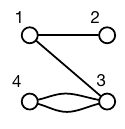
\includegraphics[width=0.3\textwidth, center]{./figures/matrix_representation.png}
            \end{minipage}
          }
        }
          child {
            node {Adjacency matrix $A(G)$
              \resizebox{\textwidth}{!}{
                \begin{minipage}[t]{8cm}
                  \begin{itemize}
                    \item a $n\times n$ matrix with entries $a_{i,j}$
                    \item where $a_{i,j}$ is the number of edges with endpoints $\{v_i, v_j\}$
                  \end{itemize}
                  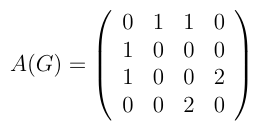
\includegraphics[width=0.3\textwidth, center]{./figures/adjacency_matrix.png}
                \end{minipage}
              }
            }
              child {
                node {Adjacency
                  \resizebox{\textwidth}{!}{
                    \begin{minipage}[t]{8cm}
                      \begin{itemize}
                        \item if $u$ and $v$ are endpoints of an edge they are \alert{adjacent} and \alert{neighbors}
                        \item one writes: $u\leftrightarrow v$
                      \end{itemize}
                    \end{minipage}
                  }
                }
              }
          }
          child {
            node {Incidence matrix $M(G)$
              \resizebox{\textwidth}{!}{
                \begin{minipage}[t]{8cm}
                  \begin{itemize}
                    \item a $n\times m$ matrix with entries $m_{i,j}$ (that means the $m$ columns are edges)
                    \item where $m_{i,j}$ is 
                    \begin{itemize}
                      \item $1$ if $v_i$ is an endpoint of $e_j$ and
                      \item $0$ otherwise
                    \end{itemize}
                  \end{itemize}
                  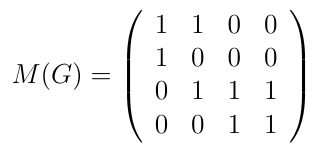
\includegraphics[width=0.3\textwidth, center]{./figures/incidence_matrix.png}
                \end{minipage}
              }
            }
              child {
                node {Incidence
                  \resizebox{\textwidth}{!}{
                    \begin{minipage}[t]{8cm}
                      \begin{itemize}
                        \item $v$ and $e$ are \alert{incident} if $v$ is an endpoint of $e$
                      \end{itemize}
                    \end{minipage}
                  }
                }
                  child {
                    node (degree) {Degree $d(v)$ or $d_G(v)$
                      \resizebox{\textwidth}{!}{
                        \begin{minipage}[t]{8cm}
                          \begin{itemize}
                            \item the \alert{degree} of vertex $v$ is the number of incident edges
                            \begin{itemize}
                              \item except for loops then the edge counts twice
                            \end{itemize}
                            \item \alert{maximum degree} is $\Delta(G)$
                            \item \alert{minimum degree} is $\delta(G)$
                            \item the number of $1$'s in a row of the incidence matrix
                          \end{itemize}
                        \end{minipage}
                      }
                    }
                  }
              }
          }
      }
      child {
        % https://latex.org/forum/viewtopic.php?t=8650
        node {Complement $\overline{G}$
          \resizebox{\textwidth}{!}{
            \begin{minipage}[t]{8cm}
            \begin{itemize}
              \item of a simple graph $G$ is the simple graph with:
              \begin{itemize}
                \item vertex set $V(G)$
                \item edge set $uv \in E(\overline{G}) \Leftrightarrow uv\not\in E(G)$
              \end{itemize}
            \end{itemize}
            \end{minipage}
          }
        }
      }
      child {
        node {Subgraph
          \resizebox{\textwidth}{!}{
            \begin{minipage}[t]{8cm}
              \begin{itemize}
                \item a \alert{subgraph }of a graph $G$ is a graph $H$ such that:
                \begin{itemize}
                  \item $V(H)\subseteq V(G)$
                  \item $E(H)\subseteq E(G)$
                  \item the assignment of endpoints to edges in $H$ is the same as in $G$
                \end{itemize}
                \item \href[page=29]{/home/areo/Documents/Studium/Summaries/Graph_Theory/Graphentheorie_english_all_in_one_with_go_back.pdf}{other definition for subgraph}
              \end{itemize}
            \end{minipage}
          }
        }
        child {
          node {Decomposition of a graph
            \resizebox{\textwidth}{!}{
              \begin{minipage}[t]{8cm}
                \begin{itemize}
                  \item germ. Kantenzerlegung (Dekomposition)
                  \item a \alert{list of subgraphs} such that \alert{a edge} appears in \alert{exactly one subgraph} in the list 
                \end{itemize}
              \end{minipage}
            }
          }
        }
          child {
            node {Clique
              \resizebox{\textwidth}{!}{
                \begin{minipage}[t]{8cm}
                  \begin{itemize}
                    \item a set of \alert{pairwise adjacent vertices}
                  \end{itemize}
                \end{minipage}
              }
            }
          }
          child {
            node (independant set) {Independant (stable) set
              \resizebox{\textwidth}{!}{
                \begin{minipage}[t]{8cm}
                  \begin{itemize}
                    \item a set of pairwise nonadjacent vertices
                  \end{itemize}
                \end{minipage}
              }
            }
          }
      }
      child {
        node {Connectivity
          \resizebox{\textwidth}{!}{
            \begin{minipage}[t]{8cm}
              \begin{itemize}
                \item a graph $G$ is \alert{connected} if each pair of vertices in G belongs to a path
                \item otherwise $G$ is \alert{disconnected}
              \end{itemize}
            \end{minipage}
          }
        }
        child {
          node {Components
            \resizebox{\textwidth}{!}{
              \begin{minipage}[t]{12cm}
                \begin{itemize}
                  \item the (connected) \alert{components} of a graph $G$ are its maximal connected subgraphs
                  \item a component is \alert{trivial} if it has no edges
                  \item an \alert{isolated} vertex is a vertex of degree $0$
                  \item every graph with $n$ vertices and k edges has at least $n-k$ components
                \end{itemize}
              \end{minipage}
            }
          }
          child {
            node {Cut-edge
              \resizebox{\textwidth}{!}{
                \begin{minipage}[t]{12cm}
                  \begin{itemize}
                    \item an edge whose deletion increases the number of components
                    \begin{itemize}
                      \item an edge is a cut-edge if and only if it belongs to no cycle
                    \end{itemize}
                  \end{itemize}
                \end{minipage}
              }
            }
          }
          child {
            node {Cut-vertex
              \resizebox{\textwidth}{!}{
                \begin{minipage}[t]{12cm}
                  \begin{itemize}
                    \item a vertex whose deletion increases the number of components
                  \end{itemize}
                \end{minipage}
              }
            }
          }
        }
      }
      child {
        node {Paths, Walks, Cycles, Circuits
          \resizebox{\textwidth}{!}{
            \begin{minipage}[t]{12cm}
              \begin{itemize}
                \item the \alert{length} is its \alert{number of edges}
              \end{itemize}
            \end{minipage}
          }
        }
          child {
            node {Walk
              \resizebox{\textwidth}{!}{
                \begin{minipage}[t]{8cm}
                  \begin{itemize}
                    \item a list $v_0, e_1, v_1, \ldots, e_k, v_k$ of \alert{vertices} and \alert{edges}
                    \begin{itemize}
                      \item for $1 \le i \le k$ the \alert{edge} $e_i$ has \alert{endpoints} $v_{i-1}$ and $v_i$
                    \end{itemize}
                    \item a \enquote{\alert{walk $W$ contains a path $P$}} if the vertices and edges of $P$ occur as a sublist of the vertices and edges of $W$
                  \end{itemize}
                \end{minipage}
              }
            }
            child {
              node {u,v-walk
                \resizebox{\textwidth}{!}{
                  \begin{minipage}[t]{8cm}
                    \begin{itemize}
                      \item \alert a {walk} with \alert{first vertex} $u$ and \alert{last vertex} $v$
                    \end{itemize}
                  \end{minipage}
                }
              }
            }
            child {
              node {Closed walk
                \resizebox{\textwidth}{!}{
                  \begin{minipage}[t]{8cm}
                    \begin{itemize}
                      \item a walk with \alert{equal first} and \alert{last vertex}
                    \end{itemize}
                  \end{minipage}
                }
              }
            }
            child {
              node {Trail
                \resizebox{\textwidth}{!}{
                  \begin{minipage}[t]{8cm}
                    \begin{itemize}
                      \item a walk \alert{without repeating edges}
                    \end{itemize}
                  \end{minipage}
                }
              }
              child {
                node {Circuit
                  \resizebox{\textwidth}{!}{
                    \begin{minipage}[t]{12cm}
                      \begin{itemize}
                        \item a \alert{closed trail}, i.e. the \alert{first} and the \alert{last vertex} are \alert{equal}
                      \end{itemize}
                    \end{minipage}
                  }
                }
              }
            }
          }
          child {
            node {Path
              \resizebox{\textwidth}{!}{
                \begin{minipage}[t]{8cm}
                  \begin{itemize}
                    \item a \alert{simple graph} whose vertices can be ordered such that:
                    \begin{itemize}
                      \item two vertices are adjacent \alert{iff} they are consecutive in the list
                    \end{itemize}
                  \end{itemize}
                  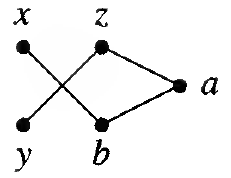
\includegraphics[width=0.3\textwidth, center]{./figures/path.png}
                \end{minipage}
              }
            }
              child {
                node {u,v-path
                  \resizebox{\textwidth}{!}{
                    \begin{minipage}[t]{8cm}
                      \begin{itemize}
                        \item a path whose vertices of \alert{degree} $1$ are $u$ and $v$ if $u\ne v$
                        \item if $u=v$ then the $u,v$-path consists only of vertex $u$ and has no edges
                      \end{itemize}
                    \end{minipage}
                  }
                }
              }
              child {
                node {Cycle
                  \resizebox{\textwidth}{!}{
                    \begin{minipage}[t]{8cm}
                      \begin{itemize}
                        \item a simple graph
                        \begin{enumerate}
                          \item with an \alert{equal} number of \alert{vertices} and \alert{edges}
                          \item whose \alert{vertices} can be placed around a \alert{circle} such that:
                          \begin{itemize}
                            \item two vertices are adjacent \alert{iff} they are consecutive in the circle
                          \end{itemize}
                        \end{enumerate}
                      \end{itemize}
                      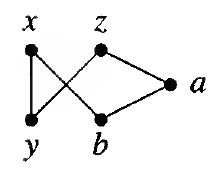
\includegraphics[width=0.3\textwidth, center]{./figures/cycle.png}
                    \end{minipage}
                  }
                }
              }
          }
      }
      child {
        node {Isomorphism
          \resizebox{\textwidth}{!}{
            \begin{minipage}[t]{8cm}
              \begin{itemize}
                \item an \alert{isomorphism} from a \alert{simple graph} $G$ to a \alert{simple graph} $H$ is a \alert{bijection} $f: V(G) \rightarrow V(H)$ such that
                \begin{itemize}
                  \item $uv\in E(G)$ \alert{iff} $f(u)f(v)\in E(H)$
                \end{itemize}
              \item one says \enquote{\alert{$G$ is isomorphic to $H$}} if there is an \alert{isomorphism} from $G$ to $H$ 
              \item one writes: $G \cong H$
              \end{itemize}
            \end{minipage}
          }
        }
      }
    }
    child {
      node {Directed Graphs / Digraphs $G = (V, E, f)$
        \resizebox{\textwidth}{!}{
          \begin{minipage}[t]{14cm}
            \begin{itemize}
              \item \alert{vertex set}, e.g. $V(G) = \{v_1, v_2, \ldots\}$
              \item \alert{edge set}, e.g. $E(G) = \{e_1, e_2, \ldots\}$
              \item a \alert{function}, .e.g. $f = \{e_1 \mapsto (v_1, v_2), \ldots\}$ assigning each edge an ordered pair of vertices
              \item the first vertex of the ordered pair is called \alert{tail}, the second vertex is called \alert{head}, together they are called the \alert{endpoints}
              \item when a digraph \alert{models a relation} each ordered pair is the pair for at most one edge. Like simple graphs we then treat the pair of endpoints as the edge
              \item in a digraph a \alert{loop} is an edge with equal endpoints
              \item \alert{multiple edges} have the same ordered pair of endpoints
              \item in an edge from $u$ to $v$
              \begin{itemize}
                \item $v$ is the \alert{successor} of $u$
                \item $u$ is the \alert{predecessor} of $v$
              \end{itemize}
              \item we write $u \rightarrow v$ for an edge from $u$ to $v$
              \item \underline{\href[page=50]{/home/areo/Documents/Studium/Summaries/Graph_Theory/Graphentheorie_english_all_in_one_with_go_back.pdf}{interesting properties}:}
              \begin{itemize}
                \item $\displaystyle \sum_{v\in V(G)} d^+(v) = e(G) = \sum_{v\in V(G)} d^-(v)$
                \item if $G$ is a digraph with $\delta^+(G)\ge 1$ or $\delta^-(G)\ge 1$ then $G$ contains a cycle
              \end{itemize}
            \end{itemize}
          \end{minipage}
        }
      }
      child {
        node {Directed Trees
          \resizebox{\textwidth}{!}{
            \begin{minipage}[t]{12cm}
              \begin{itemize}
                \item a \alert{rooted tree} $T$ is a simple digraph with a vertex $r$ chosen as root such that for each vertex $v\in V(T)$ there's a unique path \alert{$P(v)$}  from $r$ to $v$
                \item the \alert{parent} of $v\ne r$ is the predecessor in $P(v)$
                \item the \alert{children} of $v$ are the \alert{sucessor set} $N^+(v)$ of $v$
                \item the \alert{ancestors} of $v$ are all vertices of $P(v) - v$
                \item the \alert{descendants} of $v$ are all vertices $u\ne v$ such that $P(u)$ contains the vertex $v$
                \item the \alert{leaves} are vertices with no children
                \item a \alert{rooted plane tree} or \alert{planted tree} is a rooted tree with a given (left/right) ordering or labeling specified for all children of each vertex
              \end{itemize}
              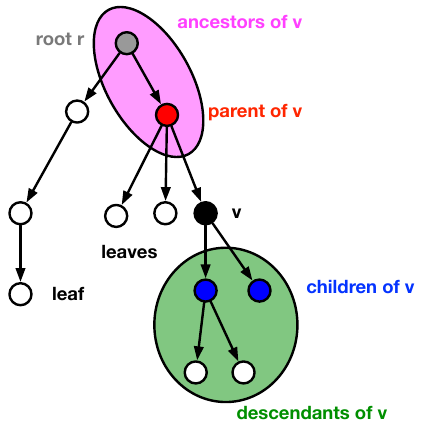
\includegraphics[width=0.6\textwidth, center]{./figures/directed_tree.png}
            \end{minipage}
          }
        }
        child {
          node {Binary Tree
            \resizebox{\textwidth}{!}{
              \begin{minipage}[t]{12cm}
                \begin{itemize}
                  \item a \alert{binary tree} is
                    \begin{itemize}
                      \item a rooted plane tree
                      \item where each vertex has at most two children
                      \item and each child of a vertex is designated as its
                        \begin{itemize}
                          \item \alert{left child} or
                          \item \alert{right child}
                        \end{itemize}
                    \end{itemize}
                  \item the subtrees rooted at the root are
                    \begin{itemize}
                      \item the \alert{left subtree} and
                      \item the \alert{right subtree}
                    \end{itemize}
                  \item a \alert{$k$-ary tree} allows each vertex up to $k$ children
                \end{itemize}
                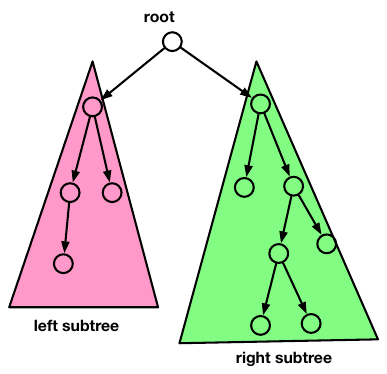
\includegraphics[width=0.6\textwidth, center]{./figures/binary_tree.png}
              \end{minipage}
            }
          }
        }
        child {
          node {Dominator Tree
            \resizebox{\textwidth}{!}{
              \begin{minipage}[t]{12cm}
                \begin{itemize}
                  \item rooted tree described by the root vertex $r$ and the edges described by $u idom v$
                \end{itemize}
              \end{minipage}
            }
          }
          child {
            node {Flowgraph
              \resizebox{\textwidth}{!}{
                \begin{minipage}[t]{12cm}
                  \begin{itemize}
                    \item a \alert{flowgraph} $G=(V,E,r)$ is 
                      \begin{itemize}
                        \item a digraph $(V, E)$
                        \item with start vertex $r$
                        \item such that for any vertex $v \in V$
                        \item there is a path from $r$ to $v$
                      \end{itemize}
                    \item a \alert{program flowgraph} is
                      \begin{itemize}
                        \item a flowgraph with maximum outdegree $2$
                      \end{itemize}
                  \end{itemize}
                \end{minipage}
              }
            }
          }
          child {
            node {Control Flow Graph (CFG)
              \resizebox{\textwidth}{!}{
                \begin{minipage}[t]{12cm}
                  \begin{itemize}
                    \item \alert{Control Flow Graph (CFG):}
                      \begin{itemize}
                        \item Given a program code $P$
                        \item each reachable line represents a vertex in the flowgraph
                        \item the first executed line is $r$ of the flowgraph
                        \item edge $(u,v)$ is in the flowgraph
                          \begin{itemize}
                            \item if and only if the control can jump from line $u$ to line $v$
                          \end{itemize}
                        \item alia for determining \alert{dominators}, i.e. Code lines guaranteed to be executed before other code
                      \end{itemize}
                    \item \alert{well structured / reducible CFG:} edges are either forward edges or back edges
                      \begin{itemize}
                        \item \alert{forward edges} form an acyclic graph reached from the entry node
                        \item \alert{back edges} consist only of edges whose targets dominate their sources
                      \end{itemize}
                  \end{itemize}
                \end{minipage}
              }
            }
          }
        }
        child {
          node {Code Tree
            \resizebox{\textwidth}{!}{
              \begin{minipage}[t]{12cm}
                \begin{itemize}
                  \item \href[page=83]{/home/areo/Documents/Studium/Summaries/Graph_Theory/Graphentheorie_english_all_in_one_with_go_back.pdf}{definition}
                  \item example \href[page=84]{/home/areo/Documents/Studium/Summaries/Graph_Theory/Graphentheorie_english_all_in_one_with_go_back.pdf}{Huffman Coding}
                \end{itemize}
              \end{minipage}
            }
          }
        }
      }
      child {
        node {Eulerian graphs
          \resizebox{\textwidth}{!}{
            \begin{minipage}[t]{12cm}
              \begin{itemize}
                \item an \alert{Eulerian trail} in a digraph (or graph) is a trail containing all edges
                \item an \alert{Eulerian circuit} is a closed trail containing all edges
                \item a digraph is Eulerian \alert{if} it has an Eulerian circuit
                \item a digraph is Eulerian \alert{iff} 
                \begin{itemize}
                  \item $d^+(v) = d^-(v)$ for all nodes $v$
                  \item the underlying graph has at most one non-trivial component
                \end{itemize}
              \end{itemize}
            \end{minipage}
          }
        }
      }
      child {
        node {Subgraphs, Isomorphism, decomposition, union
          \resizebox{\textwidth}{!}{
            \begin{minipage}[t]{12cm}
              \begin{itemize}
                \item are like in (undirected) graphs
              \end{itemize}
            \end{minipage}
          }
        }
      }
      child {
        node {Matrix representation}
        child {
          node {Incidence matrix $M(G)$
            \resizebox{\textwidth}{!}{
              \begin{minipage}[t]{12cm}
                \begin{itemize}
                  \item loopless digraph $G$
                  \item $m_{i,j} = +1$ if $v_i$ is the tail of $e_j$
                  \item $m_{i,j} = -1$ if $v_i$ is the head of $e_j$
                \end{itemize}
                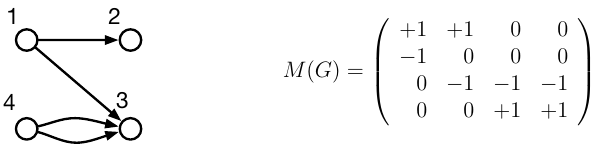
\includegraphics[width=0.8\textwidth, center]{./figures/incidence_matrix_dir.png}
              \end{minipage}
            }
          }
          child {
            node {Degree
              \resizebox{\textwidth}{!}{
                \begin{minipage}[t]{12cm}
                  \begin{itemize}
                    \item the \alert{outdegree} $d^+(v)$ is the number of edges with tail $v$
                    \item the \alert{indegree} $d^-(v)$ is the number of edges with head $v$
                    \item the \alert{out-neighborhood (successor set)} $N^+(v) := \{x \in V(G) : v \rightarrow x\}$
                    \item the \alert{in-neighborhood (predecessor set)} $N^-(v) := \{x \in V(G) : x \rightarrow v\}$
                  \end{itemize}
                \end{minipage}
              }
            }
          }
        }
        child {
          node {Adjacency matrix $A(G)$
            \resizebox{\textwidth}{!}{
              \begin{minipage}[t]{12cm}
                \begin{itemize}
                  \item digraph $G$
                  \item the entry in position $a_{i,j}$ is the number of edges from $v_i$ to $v_j$
                \end{itemize}
                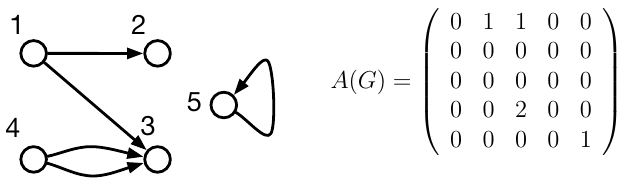
\includegraphics[width=0.8\textwidth, center]{./figures/adjacence_matrix_dir.png}
              \end{minipage}
            }
          }
        }
      }
      child {
        node {Paths, Walks, Cycles, Circuits
          \resizebox{\textwidth}{!}{
            \begin{minipage}[t]{12cm}
              \begin{itemize}
                \item the \alert{length} is its \alert{number of edges}
                \item trail, walk and circuit are the same in (undirected) graphs and digraphs
              \end{itemize}
            \end{minipage}
          }
        }
        child {
          node {Path
            \resizebox{\textwidth}{!}{
              \begin{minipage}[t]{12cm}
                \begin{itemize}
                  \item a \alert{simple digraph} whose vertices can be linearly ordered so that: 
                  \begin{itemize}
                    \item there is an edge with tail $u$ and head $v$ \alert{iff} $v$ immediately follows $u$
                  \end{itemize}
                \end{itemize}
              \end{minipage}
            }
          }
          child {
            node {u,v-path 
              \resizebox{\textwidth}{!}{
                \begin{minipage}[t]{12cm}
                  \begin{itemize}
                    \item a path whose only vertex of \alert{indegree} $0$ is $u$ and \alert{outdegree} $0$ is $v$
                  \end{itemize}
                \end{minipage}
              }
            }
          }
          child {
            node {Cycle
              \resizebox{\textwidth}{!}{
                \begin{minipage}[t]{12cm}
                  \begin{itemize}
                    \item a simple digraph whose vertices can be arranged on a circle such that: 
                      \begin{itemize}
                        \item edges exist \alert{iff} nodes follow each other according to the (without loss of generality) clockwise orientation
                      \end{itemize}
                  \end{itemize}
                \end{minipage}
              }
            }
          }
        }
        % child {
        %   node {Walk
        %     \resizebox{\textwidth}{!}{
        %       \begin{minipage}[t]{12cm}
        %         \begin{itemize}
        %           \item a list $v_0, e_1, v_1, \ldots, e_k, v_k$ of vertices and edges 
        %           \begin{itemize}
        %             \item for $1 \le i \le k$ the edge $e_i$ has tail (from) $v_{i-1}$ and head (to) $v_i$
        %           \end{itemize}
        %         \end{itemize}
        %       \end{minipage}
        %     }
        %   }
        %   child {
        %     node {Closed walk
        %       \resizebox{\textwidth}{!}{
        %         \begin{minipage}[t]{12cm}
        %           \begin{itemize}
        %             \item a walk with \alert{equal first} and \alert{last vertex}
        %           \end{itemize}
        %         \end{minipage}
        %       }
        %     }
        %   }
        %   child {
        %     node {Trail
        %       \resizebox{\textwidth}{!}{
        %         \begin{minipage}[t]{12cm}
        %           \begin{itemize}
        %             \item a walk \alert{without repeating edges}
        %           \end{itemize}
        %         \end{minipage}
        %       }
        %     }
        %     child {
        %       node {Circuit
        %         \resizebox{\textwidth}{!}{
        %           \begin{minipage}[t]{12cm}
        %             \begin{itemize}
        %               \item a \alert{closed trail}, i.e. the \alert{first} and the \alert{last vertex} are \alert{equal}
        %               \item like a circuit in computer engineering
        %             \end{itemize}
        %           \end{minipage}
        %         }
        %       }
        %     }
        %   }
        %   child {
        %     node {u,v-walk
        %       \resizebox{\textwidth}{!}{
        %         \begin{minipage}[t]{12cm}
        %           \begin{itemize}
        %             \item has \alert{first vertex} $u$ and \alert{last vertex} $v$
        %             % \item \alert a {walk} with \alert{first vertex} $u$ and \alert{last vertex} $v$
        %           \end{itemize}
        %         \end{minipage}
        %       }
        %     }
        %   }
        % }
      }
      child {
        node {Connectivity
          \resizebox{\textwidth}{!}{
            \begin{minipage}[t]{12cm}
              \begin{itemize}
                \item a digraph is \alert{weakly connected}
                \begin{itemize}
                  \item if its underlying graph is connected
                \end{itemize}
                \item a digraph is \alert{strongly connected}
                \begin{itemize}
                  \item if for each ordered pair $u$, $v$ there is a path from $u$ to $v$
                \end{itemize}
              \end{itemize}
            \end{minipage}
          }
        }
      }
      child {
        node {Types of graphs}
        child {
          node {Underlying Graph
            \resizebox{\textwidth}{!}{
              \begin{minipage}[t]{12cm}
                \begin{itemize}
                  \item The underlying graph of a digraph $D$ is the graph $G$
                  \begin{itemize}
                    \item with $V(G) = V(D)$
                    \item $E(G) = E(D)$
                    \item each ordered pairs of an edge become an unordered pair
                  \end{itemize}
                \end{itemize}
              \end{minipage}
            }
          }
        }
        child {
          node {Simple Graph
            \resizebox{\textwidth}{!}{
              \begin{minipage}[t]{12cm}
                \begin{itemize}
                  \item a digraph is simple
                  \begin{itemize}
                    \item if each ordered pair is the head and tail of at most one edge
                    \item one loop may be present at each vertex
                  \end{itemize}
                  \item in a simple digraph $uv$ denotes an edge with tail $u$ and head $v$
                \end{itemize}
              \end{minipage}
            }
          }
        }
      }
    };
  \end{scope}
  % ┌───────────────────┐
  % │ Verbindungslinien │
  % └───────────────────┘
  \begin{pgfonlayer}{background}
    \draw [concept connection]
  %     (commoncasefast) edge (amdahl)
  %     (branchpredictionbuffer) edge (2bitpredictor)
  %     (loadusedatahazard) edge (forwarding)
      (bipartite graphs) edge (independant set)
      (vc) edge (isvc)
      (vc) edge (apa)
      (regular graphs) edge (degree)
      (gt) edge (degree)
      (ec) edge (mec);
  \end{pgfonlayer}
  % ┌──────────────┐
  % │ Annotationen │
  % └──────────────┘
  % https://tex.stackexchange.com/questions/302976/node-positioning-middle-point-mind-map-connection-bar
  \node [annotation, below] at (gt.south) {This mindmap is provided without guarantee of correctness and completeness!};
  \node [annotation, below] at (gt.north) {\href{https://www.youtube.com/playlist?list=PLmsC317bB1b0m9-ZCKGNR6iM6UTPUO__r}{Recordings} where the different topics of this mindmap get explained\\\href{/tmp/current.pdf}{go back}};
  % \path (measuringexecutiontime) -- node[annotation, above, align=center, pos=0.01] {Similiar to \textbf{Response Time:} How long it takes to do a task} (ca);
  % \path (performance) -- node[annotation, above, align=center, pos=0.01] {Similiar to \textbf{Throughput}: Total work done per time unit (e.g. tasks, transactions\ldots / per hour)} (ca);
  % \path (elapsedtime) -- node[annotation, above, align=center, pos=0.01] {Also called \textbf{Wall Clock Time} or \textbf{Real Time}} (ca);
  % \path (cputime) -- node[annotation, above, align=center, pos=0.01] {Also called \textbf{User Time}} (ca);
  % % \path (branchpredictionbuffer) -- node[annotation, below, align=center, pos=-0.06] {Also called Branch History Table} (ca);
  % \path (multicycle) -- node[annotation, above, align=center, pos=0.01] {Optimize space} (ca);
  % \path (pipelining) -- node[annotation, above, align=center, pos=0.01] {Optimize time} (ca);
  \end{tikzpicture}
\end{document}
